\documentclass{article}

%%%%%%% PACKAGES %%%%%%%%
\usepackage[utf8]{inputenc}
\usepackage[margin=2cm]{geometry} %set the margin spacing
\usepackage{setspace} %1.5 line spacing
\usepackage{graphicx} %pictures
\usepackage{notoccite} %citation number ordering
\usepackage{lscape} %landscape table
\usepackage{caption} %add a newline in the table caption

\onehalfspace   % 1.5 line spacing

\title{\huge{\textbf{Progress Report - Ph.D}} \\
\LARGE{My report/thesis title here}}
\author{Joe Bloggs}
\date{June 2019}

\begin{document}
\pagenumbering{roman} % Start roman numbering
\clearpage\maketitle
\thispagestyle{empty}
\begin{center}
    \begin{figure}[h]
        \centering
        \includegraphics[width=10cm]{pics/uu_logo.png}
        %\caption{Your caption here}
        \label{fig:logo}
    \end{figure}
    \large{School of Engineering \\
    Supervisor: Prof John Smith}
\end{center}
\newpage
\setcounter{page}{1}
\tableofcontents
\listoffigures
\listoftables

\newpage
\pagenumbering{arabic} % Start roman numbering

%%% CONTENT HERE %%%%

\section{Introduction}
This document will hopefully be a start. Section \ref{Content} will show you most of what you will need.
\subsection{Content}\label{Content}
Why is report writing so difficult? This colourful plot in Figure \ref{fig:bspm} shows how body surface mapping can help detect heart attacks \cite{jennings2019}:

\begin{figure}[htbp!]
    \centering
    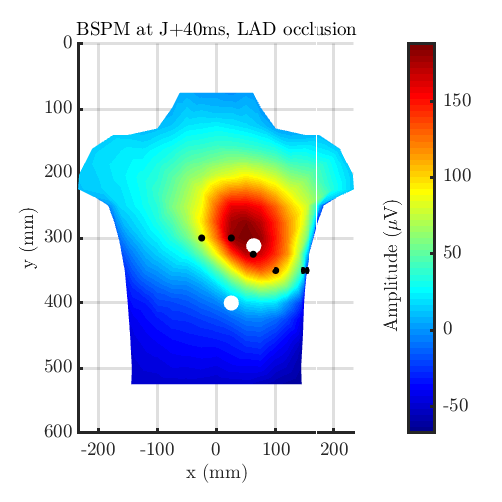
\includegraphics{pics/bspm_pbi_lad.eps}
    \caption{Anterior torso median-amplitude BSPM of sub-jects at J+40 ms during LAD occlusion PTCA (n = 14).White = SSL; black = V-leads \cite{jennings2019}}
    \label{fig:bspm}
\end{figure}

Word is suitable for quick documents or reports, however, we all must admit it is limited in professional writing. For example, academic reports, published documents and book writing involves text formatting which required huge amounts of time in Word. Table \ref{tab:time} shows how much time you can waste doing reports in Word:

\begin{table}[htbp!]
    \centering
    \def\arraystretch{1.5}%  1 is the default, change whatever you need
    \caption{Time spent using Word for each task vs LaTeX}
    \begin{tabular}{p{7cm}|p{2.5cm}|p{2.5cm}}
        Task & Time (Word) & Time (LaTeX) \\
        \hline
        Creating captioned figures & Minutes & Seconds \\
        Pretty tables & 30+ minutes & 10 minutes \\
        Page numbering the way you like it & 10 minutes & Seconds \\
        IEEE referencing across multiple chapters & Hours & Minutes
    \end{tabular}
    \label{tab:time}
\end{table}

\newpage
\setstretch{1}  %reduce bibliography line spacing
\bibliographystyle{IEEEtran}
\bibliography{references.bib}
\end{document}